\documentclass{beamer}

\iffalse
\usepackage[math]{kurier} % main font
\usepackage[utf8]{inputenc}
\usepackage[T1]{fontenc}
\fi

\usepackage[T1]{fontenc}
\usepackage[sfdefault]{FiraSans}
\usepackage[nomap]{FiraMono}


\title{Projet d'option informatique}
\subtitle{Deep Learning, traitement de langues naturelles et text mining}
\author{Damien \textsc{Douteaux} -- Vincent \textsc{Hocquemiller} -- Louis \textsc{Redonnet}}
\date{Jeudi 16 février 2017}

\usetheme{texsx}

\begin{document}

\begin{frame}[plain]
	\titlepage
\end{frame}

\section{Sommaire}

\begin{frame}
	\frametitle{Plan de la présentation}
	\tableofcontents
\end{frame}

\section{Projets envisagés}

\subsection{Analyse de liens}
\begin{frame}
	\frametitle{Présentation du sujet}
	
\end{frame}

\subsection{Reconnaissance d'auteur}
\begin{frame}
	\frametitle{Présentation du sujet}
	
\end{frame}

\subsection{Inférence}
\begin{frame}
	\frametitle{Présentation du sujet}

\end{frame}

\section{Choix du sujet}

\begin{frame}
	\frametitle{Comparaison des sujets}
	\begin{table}[ht]
		\centering
		\begin{tabular}{cccc}
			Sujet & Apports personnels & BDD & Complexité \\
			Analyse de liens & ? & Stanford & ? \\
			Reconnaissance d'auteur & Traitement du français & ? & Modérée \\
			Inférence & Traitement du français & ? & Variable \\ 
		\end{tabular}
	\end{table}
\end{frame}

\section{Base de données}

\begin{frame}
	\frametitle{Prise de contact PAr}
	\begin{itemize}
		\item Récupération de BDD
		\item Les contes
		\item Wikipédia
		\item ...
	\end{itemize}
\end{frame}


\section{Gestion de projet}

\begin{frame}
	\frametitle{Une semaine de décallage}
	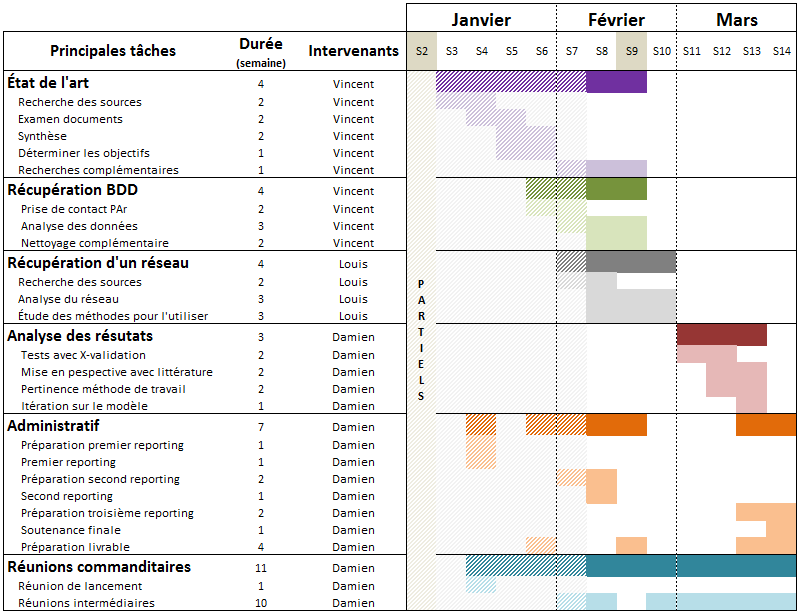
\includegraphics[height=.9\textheight]{gantt}
\end{frame}

\section{Conclusion}

\section{Références}

\begin{frame} 
	\frametitle{There is no largest prime number} 
	\framesubtitle{The proof uses \textit{reductio ad absurdum}.} 
	
	\begin{theorem}
		There is no largest prime number. 
	\end{theorem} 
	
	\begin{enumerate} 
		\item<1-| alert@1> Suppose $p$ were the largest prime number. 
		\item<2-> Let $q$ be the product of the first $p$ numbers. 
		\item<3-> Then $q+1$ is not divisible by any of them. 
		\item<1-> But $q + 1$ is greater than $1$, thus divisible by some prime
			number not in the first $p$ numbers.
	\end{enumerate}
\end{frame}

\section{Suite}
\begin{frame}{A longer title}
	\begin{itemize}
		\item one
		\item two
	\end{itemize}
\end{frame}
\end{document}
